\documentclass{article}
\usepackage[UTF8]{ctex}
\usepackage{newtxtext}
\usepackage{geometry}
\usepackage[dvipsnames,svgnames]{xcolor}
\usepackage[strict]{changepage} % 提供一个 adjustwidth 环境
\usepackage{framed} % 实现方框效果
\usepackage{setspace}
\usepackage{tikz}
\usepackage{tcolorbox}
\usepackage{amsmath}
\usepackage{graphicx}
\usepackage{wrapfig}
\usepackage{float}
\usepackage{amssymb}
\geometry{a4paper,centering,scale=0.8,left=2.0cm,right=2.0cm,top=2.0cm,bottom=2.0cm}

\definecolor{blueshade}{rgb}{0.95,0.95,1} % 文%本框颜色
\definecolor{greenshade}{rgb}{0.90,0.99,0.91} % 绿色文本框,竖线颜色设为 Green
\definecolor{redshade}{rgb}{1.00,0.90,0.90}% 红色文本框,竖线颜色设为 LightCoral
\definecolor{brownshade}{rgb}{0.99,0.97,0.93} % 莫兰迪棕色,竖线颜色设为 BurlyWood
\definecolor{yellowshade}{rgb}{1,0.945,0.7255}%米黄色
\definecolor{DarkYellow}{rgb}{0.7843,0.61176,0.0549}

\newenvironment{formal}[2][greenshade]{%
\def\FrameCommand{%
\hspace{1pt}%
{\color{#2}\vrule width 2pt}%
{\color{#1}\vrule width 4pt}%
\colorbox{#1}%
}%
\MakeFramed{\advance\hsize-\width\FrameRestore}%
\noindent\hspace{-4.55pt}% disable indenting first paragraph
\begin{adjustwidth}{}{7pt}%
\vspace{2pt}\vspace{2pt}%
}
{
\vspace{2pt}\end{adjustwidth}\endMakeFramed%
}



\title{\Huge 证券投资学-第三次作业    \\\large made by  \LaTeX}
\author{刘宇晨\hspace*{25pt}20002515\\计金(双)200}


%\begin{tcolorbox}
%    [colback=Emerald!10,colframe=cyan!40!black,title=\textbf{公式}]
%\end{tcolorbox}

\begin{document} 
\begin{figure}[H]
    \begin{center}
        
\includegraphics[width=0.3\textwidth]{logo.jpeg}
        \maketitle
    \end{center}
\end{figure}
\thispagestyle{empty}
\clearpage
\pagenumbering{arabic}
\section*{\center 第十章作业}
\subsection*{习题4}
期望收益-贝塔关系也叫做证券市场线。而这道题给出的是多因素模型。
多因素证券市场线说明对组合产生影响的每个风险因子都对其最后的总风险溢价有其贡献,
贡献量等于因子$\beta$与这一风险来源对因子组合的风险溢价的乘积。
\[E(r_P)=r_f+\beta_{P1}[E(r_1)-r_f]+\beta_{P2}[E(r_2)-r_f]\]

这道题没有给出关于两个独立经济因素的平均收益率或者风险溢价。只给了两个独立的经济因素对应投资组合
的$\beta$值和期望收益,所以可以通过这两个投资组合的多因素证券市场线来计算两个因素的风险溢价。
最后将这两个经济因素的市场溢价和无风险收益带入公式即可求得经济体的多因素证券市场线。
\nonumber
\begin{align}
    &\begin{cases}
        31\%=6\%+1.5\times R_{P1}+2\times R_{P2}\\
        27\%=6\%+2.2\times R_{P1}-0.2\times R_{P2}
    \end{cases}
    \begin{cases}
        R_{P1}=10\%\\
        R_{P2}=5\%
    \end{cases}\\
    &E(r_P)=6\%+\beta_{P1}\times 10\%+\beta_{P2}\times 5\%
\end{align}

\subsection*{习题5}
题目中所给的投资组合F的$\beta$值为0,而且是单因素投资组合,所以将其视为无风险投资。故无风险利率为6\%。

为了证明是否有套利机会,需要分别计算A和E的风险溢价与$\beta$之比。因为书中说:为了排除套利机会,期望收益率
组合的期望收益率必定会落在从无风险资产出发的直线上。这条线的方程给出了所有充分分散的投资组合的期望收益。
所以风险溢价与资产$\beta$成比例。如果两个投资组合比例不同,说明并未落在证券市场线上。
\begin{align}
    \frac{\alpha_A}{\beta_A}=(12\%-6\%)/1.2&=5\%\\
    \frac{\alpha_B}{\beta_B}=(8\%-6\%)/0.6&=3.3\%
\end{align}
所以有套利机会,下面运用两种方法进行套利。
\subsubsection*{方法1-构造$(0-\beta)$组合-灵感来自刘浩然--《CAPM模型套利问题》}
假设投资在A和E的投资比例分别为$w_A,w_E$。
\begin{align}
    \beta_z&=w_A\beta_A+(1-w_A)\beta_E=0\\
    w_A&=-1\\
    w_E&=2\\
    E(R_Z)&=w_AE(R_A)+w_BE(R_E)=\frac{\beta_A\beta_E}{\beta_A-\beta_E}(\frac{E(R_A)}{\beta_A}-\frac{E(R_B)}{\beta_B})=2.04\%
\end{align}
虽然发现$|w_A,w_E|<1$,但是我们可以通过做多投资组合E,做空投资组合A,并且(做空/做多=1/2)来投资组合$Z$。

具体套利方法:我们首先构造的投资组合$Z$的风险溢价是正的(2.04\%),我们应该做空
等比例的无风险收益(投资组合$F$)而购买投资组合$Z$,这样就可以无风险获得净利润$E(R_Z)$,并且规避掉了所有风险。


\subsubsection*{方法2-构造两个相同$\beta$的组合}
为了进行无风险套利,需要构造零净投资组合。题目中的$\beta$值均大于零,所以无法构造$\beta=0$的零净投资组合。
可以观察得出,讲投资组合$A,F$进行混合后的新投资组合的$\beta$值可以等于投资组合$E$。所以可以通过$A,F$构造新的投资组合$Z$
来构造零净投资组合。
\begin{align}
    \beta_Z&=\beta_E=0.6\\
    w\beta_A+(1-w)\beta_E&=0.6\\
    w&=0.5\\
    E(r_Z)&=0.5\times 12\%+0.5\times 6\%=9\%\\
    \alpha&=E(r_Z)-E(r_F)=9\%-8\%=1\%
\end{align}
所以两个投资组合$E,Z$具有相同的$\beta$,可以通过做多投资组合$Z$,做空投资组合$E$来进行无风险套利。
并且收益率为$\alpha =1\%$




\subsection*{习题6}
题目中说只有一个经济因素,且两个投资组合都充分分散,所以不考虑$e_i$项,
\textbf{假设两个投资组合都不存在套利机会,也就是风险溢价都为零。}运用套利定价理论的无套利等式:
\begin{align}
    E(R_P)&=\beta_PE(R_M)\\
    E(r_P)-r_f&=\beta_PE(R_M)\\
    12\%&-r_f=1.2\times (R_M-r_f)\\
    9\%&-r_f=0.8\times (R_M-r_f)\\
    \text{解得}&\begin{cases}
        r_f=3\%\\
        r_M=4.5\%
    \end{cases}
\end{align}

在初次做题时,我运用了构造证券市场线的方法。但是在检查后,发现不能用证券市场线进行求解。
因为题目中给的是两个充分分散的投资组合。而证券市场线表示的是单个证券的预期收益,
是只针对单个证券进行模拟的模型,不适用于此题。





\subsection*{习题7}
a.求期望收益率,收益的标准差

买进100万美元等权重的$\alpha=2\%$的股票,能获得2\%的超额收益。
相反,做空100美元等权重$\alpha=-2\%$的股票,也能获得2\%的正收益。
\[E=1000000\times 2\%\times 2=40000 \]

投资者在每个股票上持有100000美元,所以标准差为
\[\sigma_P=\sqrt{\sigma^2_P}=\sqrt{20\times {(100000\times 0.3)}^2}=134164\]

b.如果检验了50只股票、或者100支股票会怎样

收益率不变,标准差带入上式算得分别为84853,60000美元。
 
\subsection*{习题8}
a.计算证券A,B和C收益的方差
\begin{align}
    \sigma_P^2&=\beta_P^2\sigma_M^2+\sigma^2(e_P)\\
    \sigma_A^2&=\beta_A^2\sigma_M^2+\sigma^2(e_A)=0.8^2\times 20\%^2+25\%^2=0.0881\\
    \sigma_B^2&=\beta_B^2\sigma_M^2+\sigma^2(e_B)=1.0^2\times 20\%^2+10\%^2=0.05\\
    \sigma_C^2&=\beta_C^2\sigma_M^2+\sigma^2(e_C)=1.2^2\times 20\%^2+20\%^2=0.098
\end{align}

b.如果证券是一个充分分散的投资组合,计算超额收益方差的均值:非系统性风险趋近于0。$e(i)=0$

\textbf{个人认为题目理解有歧义,不知道要求的是BC组成投资组合的方差还是分别求B,B和C收益的方差}

b-1:如果证券A是一个充分分散的投资组合,求该投资组合的超额收益方差的均值:如果投资组合A充分分散,那么
该投资组合的公司特定方差为0。
\begin{align}
    \sigma_A^2&=\beta_A^2\sigma_M^2=0.8^2\times 20\%^2=0.0256\\
    \sigma_B^2&=\beta_B^2\sigma_M^2=0.04\\
    \sigma_C^2&=\beta_C^2\sigma_M^2=0.0576
\end{align}

b-2:B或C组成的投资组合的超额收益方差均值。假设投资在B上的比例为$w_B$,投资在C上的比例为$1-w_B$,
假设B或C组成的投资组合为$Z$
\[\sigma_Z^2=w_B\times \beta_B\sigma_M^2+w_C\times\beta_C\sigma_M^2=w_B\times 4\%+w_C\times 5.76\%\]

c.判断是否存在套利机会:由于题目中的证券B的$\beta=1$,故将$R_B$视为市场超额收益,将证券A,C带入单音素模型:
\begin{align}
    R_i&=\alpha_i+\beta_iR_M+e_i\\
    E(R_A)&=10\%=\alpha_A+ 0.8\times R_M\\
    E(R_B)&=12\%=\alpha_B+ 1.0\times R_M\\
    E(R_C)&=14\%=\alpha_C+1.2\times R_M\\
    \therefore \alpha_A&\neq \alpha_B\neq \alpha_C\neq 0
\end{align}

因为证券$A,B,C$都存在超额收益,所以存在套利机会。下面用图表分析该套利机会:

可以证明$A,B,C$不能和无风险利率构成一条直线,所以可以证存在套利机会。
\begin{figure}[H]
    \begin{center}
        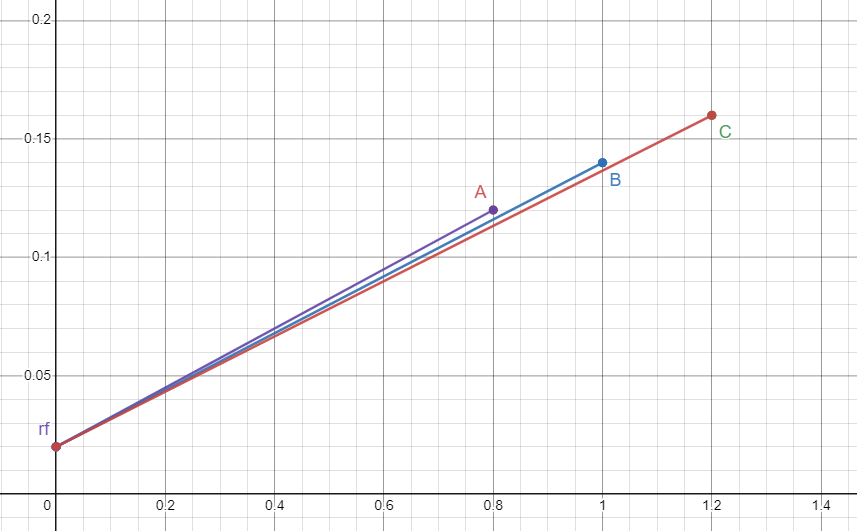
\includegraphics[width=0.43\textwidth]{2.png}\\
        \maketitle{x:$\beta$,y:收益率}
    \end{center}
\end{figure}


\clearpage
\subsection*{习题10}
 a.求股票的期望收益率:由于题目一共有三个因素,所以构造多因素模型,并求出期望收益率。
 \begin{align}
    E(r_P)&=r_f+\beta_{P1}[E(r_1)-r_f]+\beta_{P2}[E(r_2)-r_f]+\beta_{P3}[E(r_3)-r_f]\\
    E(r)&=6\%+1.2\times 6\%+0.5\times 8\% + 0.3\times 3\%\\
    &=18.1\%
 \end{align}

b.计算股票修正后的期望收益

分别对三个宏观经济因素进行分析:令通货膨胀因素为$A$,普遍认为对通货膨胀将会增长5\%,而实际上只增长4\%。
那么$A=4\%-5\%=-1\%$,代表实际增长与预期增长有-1\%的离差。同理,设宏观经济因素工业生产、石油价格分别为$B,C$。
则$B=-3\%,C=-2\%$。根据多因素模型:
\begin{align}
    E^{\prime}(r)&=E(r)-(\beta_A \times A +\beta_B \times B +\beta_C \times C )\\
    &=18.1\%-0.3\%=17.8\%
\end{align}

\subsection*{CFA考题-2}
判断投资组合X和Y是否存在套利机会。
\subsubsection*{方法一-证券市场线}
根据无风险利率为8\%($\beta = 0$),假设投资组合X期望收益率16\%为市场超额收益率($\beta =1$),构造证券市场线:
\[E(r_i)=8\%+\beta \times 8\%\]

将投资组合Y的$\beta$值带入证券市场线算得期望收益率
\begin{align}
    E(r_Y)&=8\% + \beta_Y \times 8\%\\
    &=10\%\neq E(Y)=12\%\\
    \therefore \alpha_Y&=12\%-10\%=2\%
\end{align}

由于投资组合Y不落在证券市场线上,所以选b.存在套利机会。

但是证券市场线模型只能运用于单个证券上,所以用这个方法求解不太严谨。应用单因素模型求投资组合的超额收益。
通过判断超额收益是否为零来判断是否存在套利机会。
\subsubsection*{方法二-单因素模型}
根据无风险利率为8\%,假设投资组合X期望收益率16\%为市场超额收益率的因素。由于投资组合充分分散,
所以不考虑公司特定风险,构造单因素模型:
\begin{align}
    E(R_P)&=\alpha_P+\beta_PE(R_M)\\
    E(R_Y)&=\alpha_A+0.25\times (16\%-8\%)=12\%-8\%\\
  \therefore  \alpha_Y&=2\%
\end{align}

可以算出投资组合Y的超额收益率为2\%,所以选b.存在套利机会。


\subsection*{CFA考题-3}
在什么条件下会产生正$\alpha$值的零净投资组合?(d)

\textbf{零净投资组合是指零成本进行无风险套利所运用的投资组合。}

a.投资组合的期望收益率为0:根据单指数模型回归方程
\[R_i=\alpha_i + \beta_i R_M +e_i\]
这一方程的截距$\alpha$是当市场指数超额收益率为0时该证券的期望超额收益率。如果超额收益率为0,则构造的
套利模型最终的收益率$\frac{1}{1-\beta_P}\alpha_P=0$,所以无法产生正$\alpha $的零净投资组合。

b.资本市场线是机会集的切线
我们称1月期国债和一般股票指数构成的资本配置线为资本市场线。被动策略产生于由资本市场线代表的一个投资可行集。
所以当资本市场线是机会集的切线时,只能说明这是一个最优投资组合,在资本市场线和资本配置线中并没有引入$\beta$的概念,所以不能说明可以构造零净投资组合。

c.不违背一价定律:一价定律指出:如果两项资产在所有的经济性方面均相同,那他们应该具有相同的市场价格。

根据单因素/多因素模型,可以认为经济性方面均相同的资产组合$\beta $值相同,
那么所有相同$\beta$的资产组合都具有相同的超额期望收益率,市场上不存在任何套利机会,故并不存在正$\alpha$的零净值投资组合。

d.存在无风险套利机会:如果存在无风险套利机会,那么说明存在两个投资组合,其风险溢价与$\beta $之比不相等
\[\frac{\alpha_A}{\beta_A}\neq \frac{\alpha_B}{\beta_B}\]
此时可以进行无风险套利,那么通过构造$0-\beta$模型$\frac{1}{1-\beta_P}\alpha_P$,即可构造出正$\alpha$值的零净投资组合。



\subsection*{CFA考题-4}
根据套利理论:(c)

a.高$\beta$值的股票经常被高估

b.低$\beta$值的股票经常被高估:这两个选项在第十一章的习题里有出现,为第十一章内容。

c.正$\alpha $值投资机会将很快消失:根据套利定价理论,少部分精明的套利者会将市场的套利机会消除。

d.理性投资者会从事与其风险承受度相符的套利活动:纯套利活动是无风险的,当市场上存在零风险套利机会时,理性投资者会
大量交易消除套利机会

\subsection*{CFA考题-5}
套利定价理论与单因素资本资产定价模型不同,原因在于:(d)

a.更注重市场风险:套利定价理论和单因素资本资产定价模型都是以$\beta_i$项作为市场风险项。
单因素模型描述的风险是市场风险加上公司特有风险,套利定价理论由于投资组合已经充分分散,
所以公司特有风险已经被分散,所以忽略不计,所以描述的风险只有市场风险。但是这并不表明更注重市场风险。

b.减小了分散的重要性:套利定价理论的前提条件就是充分分散投资组合。
而对于单因素模型而言,分散越大公司特有风险越低。所以分散在两个模型都很重要

c.承认多种非系统性风险因素:非系统性风险因素为公司特有风险。套利定价理论由于投资组合已经充分分散,
所以并不考虑非系统性风险,而单因素模型考虑的公司特有风险并没有考虑多种风险因素。

d.承认多种系统性风险因素:单因素模型只有一个$\beta$,即只承认一种风险因素。而套利定价理论可以有多个
$\beta$,所以承认多种系统性风险因素。

\subsection*{CFA考题-6}
当均衡价格关系被违背,投资者尽可能多地持有头寸。这是()的实例。(c)

\textbf{当均衡价格关系被违背时,市场上存在错误定价,所以有某个股票具有超额收益$\alpha$,
故存在套利机会。此时套利者会尽可能多地持有头寸,进行套利活动。}

a.支配性观点

b.均方差的有效边界

c.套利活动

d.资本资产定价模型

\subsection*{CFA考题-7}
与简单的资本资产定价模型相比,套利定价理论更具有潜在的优势,其特征为:(d)

\textbf{简单地资本资产定价模型只存在一个市场敏感指数$\beta$,而套利定价理论可以有多个$\beta$值,
可以利用多个因素对股票进行解释风险收益关系。}

a.把产量变化、通货膨胀以及利率期限结构作为解释风险收益关系的重要因素

b.按历史时间来测度无风险收益率

c.对给定的资产按时间变化来衡量套利定价理论因素的敏感性变化

d.利用多个因素而不是单因素市场指数来解释风险收益关系

\subsection*{CFA考题-8}
与资本资产定价模型相比,套利定价理论:(d)

a.要求市场均衡

b.利用基于微观变量的风险溢价

c.说明数量并确定那些能够决定期望收益率的特定因素

d.不需要关于市场投资组合的严格的假设

\clearpage
\section*{\center 第十一章作业}
\subsection*{习题12}
根据有效市场假说,下列哪些陈述是正确的(b)

\textbf{有效市场假说定义:价格能够反映所有可得到的信息}

a.未来事件能够被精准预测

b.价格能够反映所有可得到的信息

c.证券价格由于不可辨别的原因而变化

d.价格不波动
\subsection*{习题14}
如果市场是半强式有效市场,下列哪种方式是能赚取异常高交易利润的合理方式(d)

\textbf{半强式有效市场认为,与公司前景有关的全部公开的已知信息一定已经在股价中反应出来了。
但是并没有反应与企业相关的全部信息,也没有反应内幕信息。所以管理团队有先进知识的股票
可能没有被市场的价格反映出来,所以可以买入。}

a.买进低市盈率的股票:市盈率效应是低市盈率股票比高市盈率股票的投资组合的收益率更高。
通过艰苦的工作和细致分析获得超额收益完全是有可能的,但是仅凭如此简单的方法就能带来超额收益是不可能的。
并且,市盈率属于公开信息,在半强式有效市场不能利用公开信息获得异常收益。

b.买进高于近期平均价格变化的股票

c.买进低于近期平均价格变化的股票:b,c都属于技术分析,在半强式有效市场无用。

d.买进管理团队有着先进知识的股票

\subsection*{习题18}
求福特汽车公司股票价格的异常变化:市场指数上涨8\%,说明市场收益率为8\%
\begin{align}
    r_F&=0.10\%+1.1r_M\\
     &=0.10\%+1.1\times 8\%=8.9\%\\
     \therefore e_t&=7\%-8.9\%=-1.9\%
\end{align}

故福特汽车股票异常变化为-1.9\%
\subsection*{CFA考题-1}
半强有效市场假说认为股票价格(b)

\textbf{半强式有效市场认为,与公司前景有关的全部公开的已知信息一定已经在股价中反应出来了。}

a.反映了以往全部价格信息

b.反映了全部公开可得到的信息

c.反映了包括内幕消息在内的全部相关信息

d.是可预测的

\subsection*{CFA考题-2}
假定某公司宣布给持股人发放未预测的大量现金分红。在一个有效市场中,假设没有信息泄露,我们可以预测(a)。

\textbf{在有效市场中,价格反映了所有的信息。所以当信息没有泄漏的情况下,
当发红利的信息公布时会有异常价格变动}

a.在宣布时异常价格变动

b.在宣布前异常价格增加

c.在宣布后异常价格降低

d.在宣布前后没有异常价格变动

\subsection*{CFA考题-3}
下列哪一个为半强式有效市场理论提出了反对观点(d)

\textbf{在半强式有效市场中,市场价格反应了全部的信息。所以a,b,c选项都是符合半强式有效市场。
但是如果长期内低市盈率股票倾向于获得正异常收益说明投资者没有充分利用这个信息进行投资,所以是反对半强式有效市场理论的}

a.将近一半的退休金基金表现高于市场平均水平

b.所有投资者学会搜寻有关未来表现的信息

c.在确定股票价格方面交易分析是无用的

d.低市盈率股票在长期内倾向于获得正异常收益

\subsection*{CFA考题-4}
根据有效市场假说理论:(c)

\textbf{在有效市场中价格反应所有信息,所以并不存在无风险套利机会。}

a.高$\beta$股票经常被高估

b.低$\beta$股票经常被高估:对应的$\beta$会反应对应的价格,不存在高估低估问题。

c.正$\alpha$股票很快会消失

d.负$\alpha$股票对套利者来说经常获得较低收益:并不一直存在负$\alpha$股票,以为会有人通过做空负$\alpha$股票
进行套利,直至$\alpha=0$,所以异常收益会逐渐消失。
\subsection*{CFA考题-5}
下列哪种情况发生时会出现“随机漫步”(c)

\textbf{随机漫步:价格的变化是随即不可预测的。所以未来价格变化与以往价格变化无关,其他选项均有误}

a.股票价格随机变化但可以预测

b.股票价格对新旧信息均反应迟缓

c.未来价格变化与以往价格变化无关

d.以往信息对预测未来价格是有用的
\clearpage
\subsection*{CFA考题-6}
技术分析的两个基本假定是证券价格能够:(d)

\textbf{技术分析本质上是寻找股价的起伏周期和预测模式。而且成功的技术分析关键是:
股价对基本供求因素反应迟钝。所以选d}

a.根据新的信息逐步做出调整,研究经济环境能够预测未来市场的走向

b.根据新的信息迅速做出调整,研究经济环境能够预测未来市场的走向

c.根据新的信息迅速做出调整,市场价格由供求关系决定

d.根据新的信息逐步做出调整,市场价格由供求关系决定
\subsection*{CFA考题-7}
技术分析表示一只股票“相对强势”,这意味着:(a)

\textbf{在技术分析中,如果股价与某一市场指数的比率在一段时间内上升,则该股票显示了相对强势,
因为其价格表现要比大部分市场股票要好。}

a.股票价格与市场或产业指数比例倾向于上升

b.近期股票的交易量超过了正常的股票交易量

c.股票的总收益超过了国库券总收益

d.股票近期表现超过了过去表现

\end{document}



%如果投资组合的期望收益率为0,那么其必落在证券市场线之下。
%因为给定任意的$\beta , E(r)=r_f+\beta \times (r_M-r_f)$,其结果必然$>r_f>0$,如果期望收益率为0, 
%那么其$\alpha=0-E(r)<0$(该投资组合对应证券市场线上的期望收益率的相反数),所以不会产生正$\alpha$值的零净投资组合。
